\documentclass[a4paper,12pt]{report}
\usepackage{graphics}
\usepackage{graphicx}
\usepackage{textcomp}
\usepackage{array,longtable}
\usepackage{listings}
\usepackage{float}
\usepackage{color}
\usepackage{amsmath}
\usepackage{textcomp}
\usepackage{xcolor}
\usepackage{blindtext}
\usepackage{pstricks}
\usepackage{pst-node}
\usepackage{pst-grad}
\usepackage{pst-coil}
\usepackage{pst-text}
\usepackage{minted}
\usepackage{etex}
\usepackage{multicol}
\usepackage{url}
\usepackage{float}
\usepackage[letterpaper, margin=1in]{geometry}

\lstset{basicstyle=\footnotesize\ttfamily,breaklines=true}
\lstset{framextopmargin=50pt}
%%%
% \usepackage{geometry}
% \geometry{
% a4paper,
% total={170mm,257mm},
% left=20mm,
% top=20mm,
% }
%%% 
\begin{document}
 
% Title Page
\begin{titlepage}
\begin{center}
    \vspace*{\fill}
    \huge{Constraint Generation Library for LLVM}\\
    \vspace{2cm}
    \large{2017}\\


    \vspace{2cm}
    \textbf{Pushpinder Singh (14103088)}\\
    Computer Science Department,\\
    PEC University of Technology\\

    ~\\
    \textit{Under the guidance of}\\
    \textbf{Prof. Uday Khedker}\\
    Computer Science Department,\\
    IIT Bombay

    \vspace*{\fill}
\end{center}
\end{titlepage}

~\\
\vspace{2cm}
\begin{center}
\large{DECLARATION}
\end{center}
\vspace{1cm}

I here by declare that the project report entitled \textit{Constraint Generation Library for LLVM}
submitted by me to PEC University of Technology, Chandigarh in partial fullfillment of the
requirement for the award of the degree of B.Tech. in Computer Science \& Engineering is
a record of bonfide project work carried out by me under the guidance of Prof. Uday Khedker,
Department of Computer Science, IIT Bombay.
I further declare that the work reported in this project has not been submitted and will not
be submitted, either in part or in full, for the award of any other degree or diploma in this
institute or any other institute or university.

\vspace{2cm}

\begin{flushright}
Signature of the candidate\\
(Pushpinder Singh)
\end{flushright}
Date: 13 May, 2017


\begin{abstract}

This document describes constraint-gen library which helps in generating \textit{Points-to}
constraints for LLVM IR. Most of the points-to analysis depends on common
properties of pointers present in the source code. These properties for
each pointer in the source code can be gathered by using this library for
LLVM IR.

\end{abstract}

\tableofcontents

\listoftables

\chapter{Introduction}

A number of points-to analysis have been developed like Andersen's Analysis
\cite{Andersons}, Steensgaard's Pointer Analysis \cite{Steensgaard}, or Vini's
Generalizing the Liveness Based Points-to Analysis \cite{Vini:2014}, or GPG Analysis \cite{Pritams}. All these
analysis have one thing in common that they depend upon some common properties of
the pointers  present in the source code of a program. These properties include
information like the assignments to the pointers, type information, or level
of indirection. This information can represented in the form of set of constraints.
A single constraint represents a single assignment in the source code.

This library tries to extract this type of information in form of constraints 
from LLVM IR. It provides a set of well defined APIs for generating constraints 
from LLVM IR.

\section{Motivation}
Most of the points-to analyses depend only on the pointer assignments in
the source code. Other assignments for such analyses doesn't matter because
they do not affect pointers. For implementing these analyses, the
first step would be to extract these assignments. It would be quite a waste of time
to write code for the same if someone has to write a number of such analysis.
So instead of wasting time on writing code for extracting these statements,
this library provides an API for doing so easily. The implementer now only
has to focus on implementing the analysis.

This library has been designed keeping in mind the forward and backward
analysis and top-down and bottom-up analyses. So it generates constraint
without depending on the flow or context information.

\chapter{constraint-gen library}

constraint-gen library is designed to generate Points-to constraints from the
LLVM Intermediate Code. In order to generate the constraints, it classifies the
LLVM IR instructions into four primitive pointer assignments as described 
in Section 2.2. Only those LLVM IR statements are considered which are
relevant for \textit{Points-to Analysis} i.e. only those instructions in which 
there is write to a pointer location. The library treats every statement in the
program independently. Thus constraints generated are independent and are not 
affected by control flow or context. So, if someone wants to do a 
forward flow analysis or backward flow analysis, or context sensitive or 
insensitive, this library will be helpful.

\section{Design}
The library is designed such that it can cover the requirements of the most of the
points-to analysis. Every variable in the source code is represented by a single data
structure known as \texttt{PointsToNode}. Internally this library maintains a mapping 
between those \texttt{PointsToNode} and LLVM's \texttt{Value} (every variable or instruction is 
represented by this \texttt{Value}). Each \texttt{PointsToNode} is assigned a unique id. This 
id is an unsigned integer. Each constraint represents a single assignment in 
the IR. Section 2.3 discusses more about implementation level details 
of a single constraint. So instead of using the actual PointsToNode object at
multiple places only ID can be used. It also helps in debugging and keeps low
memory footprint.

\section{Classification of LLVM Instructions}
Following four basic categories are used to classify the LLVM instructions:

\begin{itemize}
    \item Address Of Instructions, e.g. a = \&b
    \item Load Instructions, e.g.  a = *b
    \item Store Instructions, e.g. *a = b
    \item Copy Instructions, e.g. a = b
\end{itemize}

Following assignments can easily modelled using the above basic statements,

\begin{table}[H]
\centering
\caption{Assignments modelled using base assignments}
\label{my-label}
\begin{tabular}{|p{5cm}|p{5cm}|p{5cm}|}
\hline

y = x-\textgreater f & y = (x-\textgreater f) & a = b \\ \hline
x-\textgreater f = y & \begin{tabular}[c]{@{}l@{}}t = \&(x-\textgreater f)\\ *t = y\end{tabular} & t = \&a; *t = b \\ \hline
y = x.f             & y = (x.f) & a = b \\ \hline
x.f = y             & \begin{tabular}[c]{@{}l@{}}t = \&(x.f)\\ *t = y\end{tabular} & t = \&a; *t = b;
\end{tabular}
\end{table}

\subsection{Address Of Instructions}
Address of instructions are those instructions which refers to the assignment 
in which address of some variable is assigned to some other variable/pointer.
Address of instruction corresponds to following standard C statement,
    
\begin{lstlisting}
    a = &b
\end{lstlisting}

In LLVM, this is satisfied by alloca and getelementptr instruction.
Alloca instruction allocates memory in the stack and returns a pointer to it.
Whereas, getelementptr instruction takes a base address and computes the address
of element relative to base address using the provided arguments.
Example,

\begin{minted}[fontsize=\footnotesize]{llvm}
%a = alloca i32, i32 4
%x = getelementptr i32, i32* %a, i32 1   ;select second element                 
\end{minted}

\noindent
First statement is equivalent to, (here b is memory being allocated in stack)

\begin{lstlisting}
    a = &b
\end{lstlisting}

\noindent
And the second statement is equivalent to,
\begin{lstlisting}
    x = &a[1]
\end{lstlisting}

\noindent
Following statements are classified as address-of instructions
\begin{itemize}
    \item \texttt{alloca}
    \item \texttt{getelementptr}
\end{itemize}

\subsection{Load Instructions}
Load instructions are those assignments in which the address stored at the 
location pointed by a pointer is assigned to another pointer.
Load instructions in LLVM can be represented using following C statement,
\begin{lstlisting}
    a = *b
\end{lstlisting}

\noindent
Load instructions in LLVM take an address and read memory from that address,
e.g.,

\begin{minted}[fontsize=\footnotesize]{llvm}
    %a = load i32*, i32** %b
\end{minted}

\noindent
Here \texttt{load} instruction will read the memory from the location pointed 
by \texttt{\%b} and will store the value read into the \texttt{\%a}.

\noindent
Instruction that satisfies this type is,
\begin{itemize}
 \item \texttt{load}
\end{itemize}


\subsection{Store Instructions}
Store instructions are those assignments in which address stored in a pointer 
is assigned to the location pointed by another pointer.
Store instructions in LLVM is equivalent to following C statement,
\begin{lstlisting}
    *a = b
\end{lstlisting}

\noindent
Store instruction in LLVM writes to the memory at address provided as second
argument. First argument is the value which has to be written.
Example,
\begin{minted}[fontsize=\footnotesize]{llvm}
    store i32* %b, i32** %a
\end{minted}

\noindent
constraint-gen library ignores those store statements which do not write address
to memory or which involves writing non pointer values to the memory. So the
following store statements in the IR will be ignored,

\begin{lstlisting}
    store i32 10, i32* %a
\end{lstlisting}

\noindent
Instruction that satisfies this type is,
\begin{itemize}
 \item \texttt{store}
\end{itemize}


\subsection{Copy Instructions}
Copy instructions are those instructions which involve copying of the address 
from one SSA variable to another. For e.g. in phi instruction
\begin{lstlisting}
    %b = phi i32* [ %a, %one ], [ %c, %two ]
\end{lstlisting}

\noindent
It is equivalent to the following C statement,
\begin{lstlisting}
    b = a;
    b = c;
\end{lstlisting}

\noindent
Following instructions satisifies this constraint,
\begin{itemize}
    \item \texttt{phi}
    \item \texttt{select}
    \item \texttt{extractvalue}
    \item \texttt{insertvalue}
\end{itemize}

More details about the constraint being generated for each instruction are
mentioned in next section.

\section{Constraints and their Generation}
Constraints are the information about the pointers assignments used in a 
particular IR statement. A single constraint refers to a single possible 
assignment. This assignment can be one of above four type. Each constraint has 
the following properties,

\begin{itemize}
    \item LHS node id
    \item RHS node id
    \item LLVM statement
    \item Type of the constraint, i.e. address of, or load, or store, or copy
\end{itemize}

\noindent
Both LHS and RHS node consists of atleast the following information. 
(Implementation details are discussed in Section 2.4).

\begin{itemize}
    \item the corresponding \texttt{llvm::Value}
    \item what other nodes are being used (See section ??)
    \item Type information, whether it is a struct or an array or a normal 
pointer
    \item A unique identifier
\end{itemize}

\subsection{Generation of constraints}
For each statement type, respective method is used to extract constraint from
that statement type. Constraints are generated for only following instructions.
Other instructions are irrevelant since they do not use pointers or involve
assignments that affect pointer locations.

\begin{itemize}
    \item \texttt{alloca} instruction
    \item \texttt{load} instruction
    \item \texttt{store} instruction
    \item \texttt{getelementptr} instruction
    \item \texttt{phi} instruction
    \item \texttt{bitcast} instruction
    \item \texttt{select} instruction
    \item \texttt{extractvalue} instruction
    \item \texttt{insertvalue} instruction
\end{itemize}

\subsubsection{\texttt{alloca} instruction}
Alloca instruction falls under the category of address-of instruction. Alloca 
instruction allocates the memory in stack taking the type and number of 
elements as arguments. It returns the pointer to that memory. 
Example,

\begin{lstlisting}
    %a = alloca i32
\end{lstlisting}
\noindent
Above instruction allocates the memory for i32 value and returns a pointer to 
it. \%a is of type i32*. Constraint that is generated will be of the following 
form,

\begin{lstlisting}
    { lhs-id } = & { rhs-id }
\end{lstlisting}
\noindent
where \texttt{lhs-id} and \texttt{rhs-id} are the id's of the variables. 
\texttt{lhs-id} represents the \texttt{\%a} and \texttt{rhs-id} represents the 
node whose address is being assigned. In LLVM, this is a virtual node. So, 
library creates a dummy node.
Example,

\begin{lstlisting}
    1 = & 0
\end{lstlisting}


\subsubsection{\texttt{load} instruction}
Only those load instructions whose return type is a pointer type are used for
generating constraint. For e.g for the following load instruction

\begin{lstlisting}
    %a = load i32*, i32** %b
\end{lstlisting}

\noindent
RHS node is \%b and LHS node is \%a. And the type of instruction is load.

\subsubsection{\texttt{store} instruction}
In case of store instruction, only those instructions are considered in which
there is write to a pointer value. For e.g.

\begin{lstlisting}
    store i32* %a, i32** %b
\end{lstlisting}
\noindent
and the following store instruction will not be considered for constraint

\begin{lstlisting}
    store i32 10, i32* %a
\end{lstlisting}

In the first example, RHS node is \%a and LHS node is \%b. And the type of 
instruction is store.

\subsubsection{\texttt{getelementptr} instruction}
getelementptr instruction in LLVM is used for calculating the address 
of a member elements of a aggregate type. So it takes the base address of
the element of an aggregate type (e.g. struct or array) as the first argument.
Indices are provided in the form of comma separated list following the base 
address.
e.g.

\begin{lstlisting}
    %a = getelementptr { i32*, i32 }, { i32*, i32 }* %b, i32 0, i32 0
\end{lstlisting}

getelementptr instruction generates special kind of constraint in which LHS is 
same as \%a but RHS is a special node consisting of list of nodes being used as 
arguments. So, LHS here is \%a, and RHS is a node consisting of \%b, `i32 0' 
and `i32 0' in its use list. Or we can say that RHS uses \%b, i32 0 and i32 0. And 
the type of instruction is copy.

\subsubsection{\texttt{phi} instruction}
Phi instruction maintains the list of all the incoming values in its use list
as its RHS. While LHS is same as in LLVM statement.
E.g.
\begin{lstlisting}
    %a = phi i32* [ %0, %one ], [ %1, %two ], [ %3, %three ]
\end{lstlisting}

Phi instruction generates multiple constraints. Each of these constraint 
consists of single possible assignment to the LHS. So the constraints generated 
for above instruction will be, \%a = \%0, \%a = \%1, \%a = \%3. Each of these 
constraints is a copy assignment.

\subsubsection{\texttt{bitcast} instruction}
bitcast instruction can convert a pointer of one type to another type. It is
essentially a copy operation. LHS be the new pointer and RHS will be the old 
pointer.

E.g.
\begin{lstlisting}
    %a = bitcast i32* %b to i64*
\end{lstlisting}

\subsubsection{\texttt{select} instruction}
select instruction is similar to br instruction. So, instead of jumping, it
selects a value from a pair based on a condition variable. It also generates 
multiple constraints where each constraint is a possible assignment. Each 
constraint represents a copy assignment.

E.g.
\begin{lstlisting}
    %c = select i1 %cond, i32* %a, i32* %b
\end{lstlisting}

Constraints generated for this instruction will be, \%c = \%a \& \%c = \%b

\subsubsection{\texttt{extractvalue} instruction}
ExtractValue instruction is used to extract the value of a member element from 
an object of an aggregate type (struct or array). Whereas getelementptr is used 
to calculate the address of a member element with respect to the base address, 
the extractvalue instruction is used to directly access the value having a 
member element. It takes the object directly as the first argument and next 
arguments are the list of indices representing the index of the member 
elements of an aggregate type.

For e.g. if \%a is of type { i32*, i32 }, then 
following instruction will extract the address being holded by first member 
which is a pointer.

\begin{lstlisting}
 %first = extractvalue { i32*, i32 } %a, 0
\end{lstlisting}

Constraint generated is similar to the that of getelementptr instruction but 
instead it is of type copy. RHS contains the \%a node and in its use list, it 
contains the indices directly. So, unlike getelementptr, it doesn't store the 
id's of the node being used because indices are constants here. But in 
getelementptr instruction, indices can be variable too.

\subsubsection{\texttt{insertvalue} instruction}
Insertvalue instruction is used to insert a value into the member element of an 
object of an aggregate type.
The first operand of an ‘insertvalue‘ instruction is a value of struct or array 
type. The second operand is a first-class value to insert. The following 
operands are constant indices indicating the position at which to insert the 
value in a similar manner as indices in a ‘extractvalue‘ instruction. The value 
to insert must have the same type as the value identified by the indices.

For e.g.,

\begin{lstlisting}
 %aggregate = insertvalue { i32*, i32 } %a, i32* %b, 0
\end{lstlisting}

The above code is similar to the following C code,

\begin{lstlisting}
 t = a;
 t.first = b;
 aggregate = t;
\end{lstlisting}

The constraint generated is of type copy as it copies the address stored in \%b 
to a member of an object of aggregate type. RHS node of the constraint will be 
same as that of insertvalue instruction.

\section{Instructions not handled}
Following instructions are not being handled by the library,

\begin{itemize}
    \item call
    \item ret
    \item inttoptr
    \item ptrtoint
\end{itemize}

\section{Examples}
This sections provides some small examples of constraints generated using the
library.

\paragraph{Example 1}

\begin{minted}[fontsize=\footnotesize]{c}
void f() {
    int a;
}
\end{minted}

\noindent
LLVM IR,
\begin{minted}[fontsize=\footnotesize]{llvm}
define void @f() {
    %a = alloca i32
    ret void
}
\end{minted}

Corresponding constraints,
\begin{lstlisting}
1 = & 0
\end{lstlisting}

\paragraph{Example 2}


\begin{minted}[fontsize=\footnotesize]{c}
void f() {
    int a;
    int *b;
    b = &a;
}
\end{minted}

\noindent
LLVM IR,
\begin{minted}[fontsize=\footnotesize]{llvm}
define void @f() {
    %a = alloca i32
    %b = alloca i32*
    store i32* %a, i32** %b
    ret void
}
\end{minted}

Corresponding constraints,
\begin{lstlisting}
1 = & 0
3 = & 2
* 3 = 1
\end{lstlisting}

\paragraph{Example 3}

\begin{minted}[fontsize=\footnotesize]{c}
void f() {
    int *b;
    b;
}
\end{minted}

\noindent
LLVM IR,
\begin{minted}[fontsize=\footnotesize]{llvm}
define void @f() {
    %b = alloca i32*
    %1 = load i32*, i32** %b
    ret void
}
\end{minted}

Corresponding constraints,
\begin{lstlisting}
1 = & 0
2 = * 1
\end{lstlisting}

\paragraph{Example 4}

\begin{minted}[fontsize=\footnotesize]{c}
struct A {
    int *x;
    int y;
};

void foo() {
    struct A a;
    int b;
    a.x = &b;

}
\end{minted}

\noindent
LLVM IR,
\begin{minted}[fontsize=\footnotesize]{llvm}
define void @foo() {
    %a = alloca { i32*, i32 }
    %b = alloca i32
    %1 = getelementptr { i32*, i32 }, {i32*, i32}* %a, i32 0, i32 0
    store i32* %b, i32** %1
    ret void
}
\end{minted}

Corresponding constraints,
\begin{lstlisting}
1 = & 0
3 = & 2
6 = & 4 uses: { 1, 5, 5 }
* 6 = 3
\end{lstlisting}

\paragraph{Special Example 1}

\begin{minted}[fontsize=\footnotesize]{c}
void f() {
    int *a = nullptr;
}
\end{minted}

\noindent
LLVM IR,

\begin{minted}[fontsize=\footnotesize]{llvm}
define void @foo() {
    %a = alloca i32*
    store i32* null, i32** %a
    ret void
}
\end{minted}

\noindent
Corresponding constraints,

\begin{lstlisting}
1 = & 0
* 1 = 2
\end{lstlisting}

In the above example, LLVM uses special keyword for representing null pointers.
This null is different for every pointer type. So \texttt{i32* null} is different
from \texttt{i32** null}.

\paragraph{Special Example 2}
\begin{minted}[fontsize=\footnotesize]{c}
void f() {
    int *a = (int*)malloc(sizeof(int));
}
\end{minted}

\noindent
LLVM IR,

\begin{minted}[fontsize=\footnotesize]{llvm}
define void @f() {
entry:
  %a = alloca i32*
  %call = call i8* @malloc(i64 4)
  %0 = bitcast i8* %call to i32*
  store i32* %0, i32** %a
  ret void
}

\end{minted}

\noindent
Corresponding constraints,

\begin{lstlisting}
    1 = & 0
    2 = 3
    * 1 = 2

    where,
    0: DummyNode
    1: %a
    2: %0
    3: %call
\end{lstlisting}

\section{Globals handling}
Global variables define regions of memory allocated at compilation time instead
of run-time. Global variables always define a pointer to their ``content'' type
because they describe a region of memory, and all memory objects in LLVM are
accessed through pointers. For e.g. following examples creates a global integer.

\begin{minted}[fontsize=\footnotesize]{llvm}
    @g = global i32 0 
\end{minted}


\noindent
Here \texttt{@g} has type \texttt{i32*}.

In IR, globals are used just like another pointers. Except they have prefix of
``@'' instead of usual ``\%''.

\noindent
Some examples,
\begin{minted}[fontsize=\footnotesize]{c}
int a = 10;
int *b;

int main() {
    int *c = &a;
    b = c;
    return 0;
}
\end{minted}

\noindent
LLVM IR,

\begin{minted}[fontsize=\footnotesize]{llvm}
@a = global i32 10
@b = common global i32* null

define i32 @main() {
entry:
  %retval = alloca i32, align 4
  %c = alloca i32*, align 8
  store i32 0, i32* %retval, align 4
  store i32* @a, i32** %c, align 8
  %0 = load i32*, i32** %c, align 8
  store i32* %0, i32** @b, align 8
  ret i32 0
}
\end{minted}

\noindent
Corresponding constraints,

\begin{lstlisting}
    1 = & 0
    3 = & 2
    * 3 = 4
    5 = * 3
    * 6 = 5

where,
0: DummyNode
1: %retval
2: DummyNode
3: %c
4: @a
5: %0
6: @b
\end{lstlisting}

\chapter{Implementation Details}
In this chapter, implementation level details of this library are provided. Various 
data structures used and important APIs are explained in the following sections.

The whole project is maintained using git. Project repository is hosted using
GitHub \cite{GitHub}. Following is the directory structure of the project,

\begin{itemize}
  \item cmake/      Important cmake modules required for building library
  \item docs/       Documentation
  \item include/    The public interface to the library
  \item samples/    Sample C code for testing and debugging
  \item src/        Implementation of the library
  \item tests/      Test code
  \item utils/      Small utility libraries
\end{itemize}

\section{Data Structures}
In this section, various classes and their properties used in the library are 
explained.

\subsection{\texttt{PointsToNode}}
This is an important class which holds the information regarding single 
pointer/variable. Though as the name suggests that this class represents 
pointers only, but in some cases it can represent non-pointers as well.
Every object of this class is assigned a unique id. This id is used in place 
of using object directly. Thus helps in easier debugging. Class details are provided in Table \ref{points-to-node}.

\begin{table}[]
\centering
\caption{PointsToNode}
\label{points-to-node}
\begin{tabular}{|l|l|l|}
\hline
getValue     & llvm::Value*  & returns the corresponding llvm::Value object.                               \\ \hline
getType      & llvm::Type*   & Returns the pointer to llvm::Type                                           \\ \hline
hasStructTy  & bool          & Returns true if this node has struct type.                                  \\ \hline
hasArrayTy   & bool          & Returns true if this node has array type.                                   \\ \hline
hasPointerTy & bool          & Returns true if this node has pointer type                                  \\ \hline
getId        & NodeIndex     & Returns the ID of this node                                                 \\ \hline
use\_begin   & use\_iterator & Returns iterator to beginning of use list                                   \\ \hline
use\_end     & use\_iterator & Returns iterator to the one past last element of the use\_list              \\ \hline
use\_size    & size\_t       & Returns the size of the use list.                                           \\ \hline
use\_empty   & bool          & Returns true if use list is empty                                           \\ \hline
getUse       & NodeIndex     & Returns nth use.                                                            \\ \hline
isDummy      & bool          & Returns true if this node is a dummy node.                                  \\ \hline
dump         & void          & Dumps this node to the provided llvm::raw\_ostream object.                  \\ \hline
\end{tabular}
\end{table}



\subsection{\texttt{NodeIndex}}
This type is used for ID's. Every \texttt{PointsToNode} object is assigned
a unique ID of type \texttt{NodeIndex} which is equivalent to \texttt{unsigned int}.

\subsection{\texttt{Constraint}}
This class holds the information of single possible assignment in an 
instruction. It holds the id's of two PointsToNode objects and the type of the 
assignment which can be one of the four possible assignments as described 
in Section 2.2. Details about member functions are provided in Table \ref{constraint}.

\begin{table}[]
\centering
\caption{Constraint}
\label{constraint}
\begin{tabular}{|l|l|l|}
\hline
getLHSId                    & NodeIndex      & returns the ID of the LHS node            \\ \hline
getRHSId                    & NodeIndex      & returns the ID of the RHS node            \\ \hline
getType                     & ConstraintType & returns the type of constraint            \\ \hline
dump                        & void           & dumps the constraint to the stream object \\ \hline
\end{tabular}
\end{table}

\subsection{\texttt{ConstraintBuilder}}
This class provides APIs for generating constraints from LLVM IR. This class 
also provides public methods to generates ID's for LLVM pointers. Details about member functions of this class are provided in Table \ref{constraint-builder}.

\begin{table}[]
\centering
\caption{ConstraintBuilder}
\label{constraint-builder}
\begin{tabular}{|l|l|p{8cm}|}
\hline
getConstraint  & std::vector\textless Constraint\textgreater & takes an llvm::Instruction pointer and returns a list of constraints. \\ \hline
generateId     & NodeIndex                                  & takes an llvm::Value pointer and returns the ID of that value.        \\ \hline
makeConstraint & Constraint                                 & creates a Constraint object.                                          \\ \hline
\end{tabular}
\end{table}

\subsection{\texttt{PointerSymbolTable}}
This class manages all the tables and various mappings between library's 
objects and LLVM's objects. This class is used by ConstraintBuilder in order to 
generate ID's. Member details of this class are in Table \ref{pointer-symbol-table}.

\begin{table}[]
\centering
\caption{PointerSymbolTable}
\label{pointer-symbol-table}
\begin{tabular}{|l|l|p{8cm}|}
\hline
getValue & PointsToNode* & returns a PointsToNode object corresponding to an ID. \\ \hline
createPointerNode & NodeIndex & creates a new PointsToNode object and stores it in a map and returns the ID of that object. \\ \hline
size & size\_t & returns the size of the table. \\ \hline
dump & void & prints the table to the llvm::raw\_ostream object. \\ \hline
createDummyNode & NodeIndex & creates a dummy PointsToNode object in the map. These objects don't have any llvm::Value. \\ \hline

\end{tabular}
\end{table}

\paragraph{}
More details about each class' members and public methods are described in 
documentation generated by doxygen from source directly.

\section{Public APIs}
\texttt{ConstraintBuilder} class provides interface for generating constraints
and generating ID's for LLVM IR. These methods are described below.

\subsection{\texttt{getConstraint}}
\paragraph{Prototype}
\begin{minted}[fontsize=\footnotesize]{C++}
std::vector<Constraint>
    getConstraint(llvm::Instruction *i);
\end{minted}

\paragraph{Description:}
This function takes pointer to the LLVM Instruction object and generates a list
of constraints. For most of the instructions, except some copy instructions,
this only generates single constraint. It returns the list of constraints. If
the list is empty then it means that instructions was invalid for generating
constraint.

\subsection{\texttt{generateId}}
Since the library does not handles \texttt{call/invoke} instructions so it provides
this function for assigning ID's to the LLVM variables which were missed in the call
instruction by the library.

\paragraph{Prototype}
\begin{minted}[fontsize=\footnotesize]{C++}
NodeIndex generateId(llvm::Value *val);
\end{minted}

\paragraph{Description:}
This function takes a pointer to LLVM Value object and creates a \texttt{PointsToNode}
object and returns the ID of that object.

\subsection{\texttt{makeConstraint}}
\paragraph{Prototype}
\begin{minted}[fontsize=\footnotesize]{C++}
Constraint makeConstraint(NodeIndex lhs,
                          NodeIndex rhs,
                          ConstraintType type);
\end{minted}

\paragraph{Description}
This function takes three arguments. First two are the ID's of the lhs and rhs
respectively and the last argument is the \texttt{ConstraintType} which can be
one of the following:
\begin{itemize}
    \item \texttt{kInvalid}
    \item \texttt{kAddressOf}
    \item \texttt{kLoad}
    \item \texttt{kStore}
    \item \texttt{kCopy}
\end{itemize}

\chapter{Using this library}
This section discusses about how to use this library for implementing an analysis.
The library can be integrated into project by two ways,

\begin{itemize}
    \item Developing Analysis inside the source tree of constraint-gen library.
    \item Integrating constraint-gen library inside the source tree of the analysis.
\end{itemize}

\section{Developing Analysis inside the source tree of constraint-gen library}
If analysis is small, then it can be simply written inside the source tree
of the constraint-gen library. The source files will remain inside \texttt{tests/}
directory. Then add the following line to the \texttt{tests/CMakeLists.txt}

\begin{minted}{cmake}
add_points_to_project(NameOfYourAnalysis Analysis.cc)
\end{minted}

Then compile the library. The analysis will be compiled along side library.
And \texttt{libNameOfYourAnalysis.so} will be built. Now this pass can be used
from opt as,

\begin{minted}{shell}
opt -load build/lib/libNameOfYourAnalysis.so -your-analysis-option test.ll
\end{minted}

Examples have been provided in the \texttt{tests} directory.

\section{Example pass}
\begin{minted}[fontsize=\footnotesize]{c++}
#include "llvm/Pass.h"
#include "llvm/Support/ErrorHandling.h"
#include "llvm/IR/Function.h"
#include "llvm/IR/Instructions.h"
#include "llvm/Support/raw_ostream.h"

#include "ConstraintBuilder.h"

/* For storing the constraints */
#include <vector>

using namespace llvm;
using namespace ptsto;

namespace {

struct ConstraintGen : public ModulePass {
    static char ID;

    std::vector<Constraint> constraints_;

    void print(raw_ostream &os, const Module */**/) const override {
        for (const auto &constraint : constraints_) {
            constraint.dump(os);
        }
    }

    ConstraintGen() : ModulePass(ID) { }

    bool runOnModule(Module &module) override {
        ConstraintBuilder builder;

        for (Function &f : module) {
            for (BasicBlock &bb : f) {
                 for (Instruction &i : bb) {
                    Constraint c = builder.getConstraint(&i);
                    if (c == kInvalidConstraint) {
                        continue;
                    }

                    constraints_.push_back(c);
                }
            }
        }
        return false;
    }
};

}

// static
char TestPass:ID = 0;

// registration of pass
static RegisterPass<TestPass> X("test-pass", // command line option
                                "A short description",
                                false, // looks at CFG only
                                false  // doesn't modify anything
                                );
\end{minted}

\section{Integrating constraint-gen library inside the source tree of the analysis}
In case analysis is large, then the constraint-gen library can be included directly inside
the source tree of the analysis. But this involves writing all the CMakeLists.txt files.
An example of this way can be seen in the implementation of the GPG analysis by Binapani Beria \cite{Bina}.
Best way is to use git and keep the library as a separate submodule. In this way,
updates to the library would be easier to integrate.

\chapter{Conclusion}
LLVM is great tool for program analysis. 
constraint-gen library helps in implementing the \textit{Points-to Analysis} by
providing base constraints for LLVM IR. The library can reduce the time and effort
of the developer. This library covers the base requirements of most of the
Points-to Analyses.

This library has been used in implementing a part of Pritam's GPG Analysis
\cite{Pritams}. Library has been well tested using LLVM Testing Suite.
Almost all the test cases have been covered. Its data structures are unit
tested using Google Test Framework \cite{Gtest}.

There are still few cases, where the constraints will be missed.
In case of \texttt{ptrtoint} and \texttt{inttoptr} instruction, constraints
will be missed. For example, if a pointer is casted to an integer and then casted
back to pointer then there will be information missing about the operations on that
integer.

\chapter{Appendix}
\appendix

\section{Writing a pass in LLVM}
This section describes how to write an LLVM pass.

\subsection{Writing a simple Hello World pass}
Example shown here is taken from LLVM's official documentation on writing pass \cite{llvm-pass}. 
In your pass directory, create the following CMakeLists.txt file,

\begin{minted}[fontsize=\footnotesize]{cmake}
cmake_minimum_required(VERSION 3.1)

find_package(LLVM CONFIG REQUIRED)
list(APPEND CMAKE_MODULE_PATH "${LLVM_CMAKE_DIR}")
include(LLVMConfig)

add_library(HelloWorldPass MODULE
            HelloWorldPass.cc
)

include_directories(${LLVM_INCLUDE_DIRS})
add_definitions(${LLVM_DEFINITIONS})

target_compile_features(HelloWorldPass PRIVATE cxx_range_for cxx_auto_type)

set_target_properties(HelloWorldPass PROPERTIES
    COMPILE_FLAGS "-fno-rtti -g"
)
\end{minted}

Every pass written for LLVM inherits from one of the \texttt{ModulePass}, \texttt{FunctionPass},
\texttt{BasicBlockPass} or \texttt{CallGraphPass}. It depends on what your pass is doing. This example
writes a pass that runs over function hence it inherits from \texttt{FunctionPass}.
It runs over every function and prints the name of the function to the terminal.

Following is the code for the HelloWorldPass.cc,

\begin{minted}[fontsize=\footnotesize]{c++}
#include <llvm/IR/Instruction.h>
#include <llvm/Pass.h>
#include <llvm/IR/Function.h>
#include <llvm/Support/raw_ostream.h>

using namespace llvm;

namespace {

// A simple hello world pass that prints hello: <name of function>
struct HelloWorldPass : FunctionPass {
    static char ID;

    HelloWorldPass() : FunctionPass(ID)
    { }

    bool runOnFunction(Function &function) override {
        errs() << "Hello: " << function.getName() << "\n";
        return false;
    }
};

char HelloWorldPass::ID = 0;

}

RegisterPass<HelloWorldPass> X("hello",
                                "Simple hello world pass",
                                false,
                                false);

\end{minted}

This pass can be compiled by following steps,
\begin{minted}[fontsize=\footnotesize]{shell}
mkdir build
cd build
cmake ..
\end{minted}

\texttt{libHelloWorldPass.so} will be built in the \texttt{build} directory. This pass
can be loaded into the LLVM using the \texttt{opt} tool provided in the LLVM package.

Command to run this pass,
\begin{minted}[fontsize=\footnotesize]{shell}
opt -load ./libHelloWorldPass.so -hello a.ll
\end{minted}

This pass will run for every function in a.ll by LLVM and will output the name of
the function to the terminal.

\subsection{Writing an LLVM pass that counts the number of instructions}
In this section, the hello world pass written in the previous section will be extended
to count the number of instructions present in the source code.

\begin{minted}[fontsize=\footnotesize]{c++}
#define DEBUG_TYPE "counter"
#include <llvm/Pass.h>
#include <llvm/IR/Function.h>
#include <llvm/IR/Instruction.h>
#include <llvm/ADT/Statistic.h>

using namespace llvm;

// STATISTIC is an LLVM API for doing stats related functions
STATISTIC(counter, "Number of instructions");

namespace {
// simple pass that counts the number of instructions in the IR
// use -stats option to print the number
struct CountInstructionsPass : public BasicBlockPass {
    static char ID;

    CountInstructionsPass() : BasicBlockPass(ID) { }

    bool runOnBasicBlock(BasicBlock &bb) override {
        for (const auto &i : bb) {
            counter++;
        }
        return false;
    }
};

char CountInstructionsPass::ID = 0;

}

RegisterPass<CountInstructionsPass> X("count_instructions",
                                    "Counts the number of instructions",
                                    false,
                                    false);

\end{minted}

This pass can be run as follows,

\begin{minted}[fontsize=\footnotesize]{shell}
opt -load ./libHelloWorldPass -count_instructions -stats a.ll
\end{minted}

This will count the number of instructions present in the a.ll module. \texttt{-stats} option
will print the number on the terminal.

\subsection{Writing an LLVM pass that runs on call graph}
This section describes important LLVM API's that can be used to access the call graph.
LLVM provides \texttt{CallGraphSCCPass} which can be used as to traverse the call graph
in bottom-up manner \cite{llvm-call-graph}.

\begin{quote}
\textit{The \texttt{CallGraphSCCPass} is used by passes that need to traverse the program bottom-up on the call graph (callees before callers). Deriving from \texttt{CallGraphSCCPass} provides some mechanics for building and traversing the CallGraph, but also allows the system to optimize execution of \texttt{CallGraphSCCPass}es. If your pass meets the requirements outlined below, and doesn’t meet the requirements of a FunctionPass or BasicBlockPass, you should derive from \texttt{CallGraphSCCPass}.
\\
To be explicit, \texttt{CallGraphSCCPass} subclasses are:\\
\hspace{15pt}... not allowed to inspect or modify any Functions other than those in the current SCC and the direct callers and direct callees of the SCC.\\
\hspace{15pt}... required to preserve the current CallGraph object, updating it to reflect any changes made to the program.\\
\hspace{15pt}... not allowed to add or remove SCC’s from the current Module, though they may change the contents of an SCC.\\
\hspace{15pt}... allowed to add or remove global variables from the current Module.\\
\hspace{15pt}... allowed to maintain state across invocations of runOnSCC (including global data).\\
\\
Implementing a \texttt{CallGraphSCCPass} is slightly tricky in some cases because it has to handle SCCs with more than one node in it. All of the virtual methods described below should return true if they modified the program, or false if they didn’t.
}
\end{quote}

Following is a simple example of using \texttt{CallGraphSCCPass} to traverse the call-graph of llvm.

\begin{minted}[fontsize=\footnotesize]{c++}
#include <llvm/Analysis/CallGraphSCCPass.h>
#include <llvm/Analysis/CallGraph.h>
#include <llvm/IR/Argument.h>
#include <llvm/IR/Function.h>
#include <llvm/IR/Module.h>
#include <llvm/Pass.h>
#include <llvm/Support/raw_ostream.h>

using namespace llvm;

class SimplePass : public CallGraphSCCPass {
public:
    static char ID;

    SimplePass() : CallGraphSCCPass(ID) {}

    bool runOnSCC(CallGraphSCC &SCC) override {
        for (CallGraphNode *node : SCC) {
            if (node->getFunction() == nullptr)
                continue;

            errs() << node->getFunction()->getName() << "\n";
         }
    }
};
char SimplePass::ID = 8;

static RegisterPass<SimplePass> gpganalysis("simple",
                                             "Simple pass to traverse call graph",
                                             false, false);
\end{minted}

Above pass traverses the call graph in a bottom-up manner and prints the name of the functions.

\section{Google C++ Testing Framework}
Google C++ Testing Framework \cite{Gtest} is a unit testing framework designed by google for easier
testing of C++ code. Tests written using this framework are,

\begin{itemize}
    \item Independent and Repeatable
    \item Well organized
    \item Portable and Reusable
    \item Provides much information if a test fails
    \item Fast
\end{itemize}

To write a test program using Google Test, first compile Google Test
into a library and link the test with it.

Test uses assertions, statements that check whether a condition is true or not,
to verify the tested code's behavior. An assertion's result can be success, nonfatal
failure or fatal failure. If a fatal failure occurs, the framework aborts the function;
otherwise the program continues.

A test case contains one or many tests. Tests can be grouped into test cases
that reflect the structure of the tested code. When multiple tests in a test case
need to share common objects and subroutines, then tests can be put into
a test fixture class.

Much of the details are provided in the online documentation on the project website
\cite{Gtest}.

\subsubsection{Example}
Consider a function \texttt{Factorial} which needs to be tested,

\begin{minted}[fontsize=\footnotesize]{c++}
int Factorial(int n); // Returns the factorial of n
\end{minted}

A test case for this function will look like,

\begin{minted}[fontsize=\footnotesize]{c++}
// Tests factorial of 0.
TEST(FactorialTest, HandlesZeroInput) {
  EXPECT_EQ(1, Factorial(0));
}

// Tests factorial of positive numbers.
TEST(FactorialTest, HandlesPositiveInput) {
  EXPECT_EQ(1, Factorial(1));
  EXPECT_EQ(2, Factorial(2));
  EXPECT_EQ(6, Factorial(3));
  EXPECT_EQ(40320, Factorial(8));
}
\end{minted}

\section{Type iteration in LLVM}
LLVM provides a set of API's to iterate over types. Type can be
recursive in LLVM. The instances of the Type class are immutable: once they are
created, they are never changed. Also note that only one instance of a
particular type is ever created. Thus seeing if two types are equal is a matter
of doing a trivial pointer comparison. Consider the following type,

\begin{minted}[fontsize=\footnotesize]{c}
struct A {
    int x;
    char ch;
};

struct B {
    struct A a;
    int y;
};
\end{minted}

Below is the LLVM representation,
\begin{minted}[fontsize=\footnotesize]{llvm}
%structA = type { i32, i8 }
%structB = type { %structA, i32 }
\end{minted}

Here is the visual representation of the above type,

\begin{center}
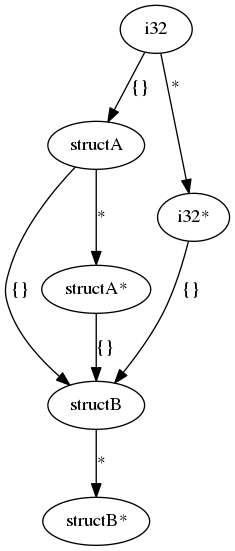
\includegraphics[scale=0.5]{output}
\end{center}

\noindent
So the simple graph traversal algorithm can be used for iterating on the
subtypes.

\noindent
For e.g below is the code for traversal over above type

\begin{minted}[fontsize=\footnotesize]{c++}
    std::set<Type*> visited_;

    void printSubType(Type *type) {
        errs() << *type << "\n";

        for (Type *subtype : type) {
            printSubType(subtype);
        }
    }

\end{minted}

\bibliography{References}
\bibliographystyle{ieeetr}
\end{document}
